\part{Lezioni di Maurizio Pratelli}

\chapter{Variabili Aleatorie con densità (continue)}

\section{Introduzione alle Variabili Aleatorie con Densità}

\begin{defn}
    \textbf{Variabile Aleatoria}
    Abbiamo visto nella parte precedente del corso le variabili aleatorie.
    Una variabile aleatoria è una funzione definita come


    \begin{equation*}
        X: (\Omega, \mathbb{F}, P) \to \R
    \end{equation*}

    Permette di trasportare le probabilità dai sottoinsiemi di $ \Omega $ ai sottoinsiemi di $ \R $, ovvero


    \begin{equation*}
        \begin{aligned}
            \text{P}_X(A) = \p{X^{-1} (A)} \\
            A \subseteq \R \\
            X^{-1}(A) \subseteq \Omega
        \end{aligned}
    \end{equation*}

    Le variabili aleatorie possono essere di \textbf{discrete}, \textbf{con densità} o \textbf{più generali}.
    Una variabile aleatoria è discreta se la sua immagine è finita o numerabile, ovvero


    \begin{equation*}
        p(x_i) = \p{X=x_i}
    \end{equation*}
\end{defn}


\begin{defn}
    \textbf{Variabile Aleatoria con Densità} \\
    $ X $ ha densità se esiste una funzione $ f : \R \to [0, +\infty) $ (la densità) integrabile, tale che

    \begin{equation*}
        \begin{aligned}
            \p{X \in A} = \int_A f(x)dx \\
            \p{a \leq X \leq b} = \int_a^b f(x)dx
        \end{aligned}
    \end{equation*}
\end{defn}

\begin{defn}
    \textbf{Funzione di ripartizione (cumulative distribution function)} \\
    È una funzione definita come $ F : \R \to [0,1]$
    È definita come
    \begin{equation}
        F_X(x) = \p{X \leq x}
    \end{equation}
    Se ne inferisce che la probabilità che la variabile aleatoria con densità $ X $
    risieda nell'intervallo semichiuso $(a,b]$ con $ a \leq b $ è quindi
    \begin{equation}
        \p{a \leq X \leq b} = \p{X \leq x}
    \end{equation}

    Sulle \textbf{variabili discrete} è tipicamente discontinua, definita come
    \begin{equation}
        F_x(t) = \sum_{x_i \leq t} \p{X = x_i} = \sum_{x_i \leq t} p(x_i)
    \end{equation}

    \textbf{Funzione di ripartizione su variabili con densità}
    Sulle \textbf{variabili con densità} è tipicamente continua e può essere espressa come
    l'integrale della funzione di densità di probabilità della variabile come segue:
    \begin{equation}
        F_X(t) = \int_{-\infty}^{t} f(x) dx
    \end{equation}
\end{defn}

\begin{exmp}
    \textbf{Densità uniforme su [a, b]} \\
    Sia data $ X $ con densità $ f $
    \begin{equation*}
        f(x) = \begin{cases}
            \frac{1}{b-a} & a \leq x \leq b \\
            0   &    \text{altrimenti}
        \end{cases}
    \end{equation*}

    % TODO grafico
    La funzione di ripartizione $F$ è definita come
    \begin{equation*}
        F(x) = \int_{-\infty}^x f(t) dt = \begin{cases}
            0 & x \leq a \\
            \frac{x-a}{b-a} & a < x < b \\
            1 & x \geq b
        \end{cases}
    \end{equation*}
    $ F $ è la funzione di ripartizione in tutti i punti in cui $ f $ è continua
    \begin{equation*}
        f(x) = \frac{dF(x)}{dx}
    \end{equation*}
\end{exmp}

\begin{exmp}
    \textbf{Densità esponenziale di parametro} $ \lambda > 0 $ \\
    Sia data la densità
    \begin{equation*}
        f(x) = \begin{cases}
            \lambda e^{-\lambda x} & x \geq 0 \\
            0 & x < 0
        \end{cases}
    \end{equation*}

    \begin{figure}[htbp]
        \centering

        \begin{tikzpicture}[
            declare function={
                func(\x,\lambda) = (\lambda*e^(-\lambda*\x))
                ;
            }]
            \begin{axis}[xlabel=$x$]
                \addplot[blue][domain=0:5] {func(x,0.5)};
                \addplot[red][domain=0:5] {func(x,1)};
            \end{axis}
        \end{tikzpicture}
        \caption{Densità di probabilità esponenziale di parametro $\lambda = 0.5$ (blu) e $\lambda = 1$ (rosso)}
        \label{exparam}
    \end{figure}

    \begin{figure}[htbp]
        \centering

        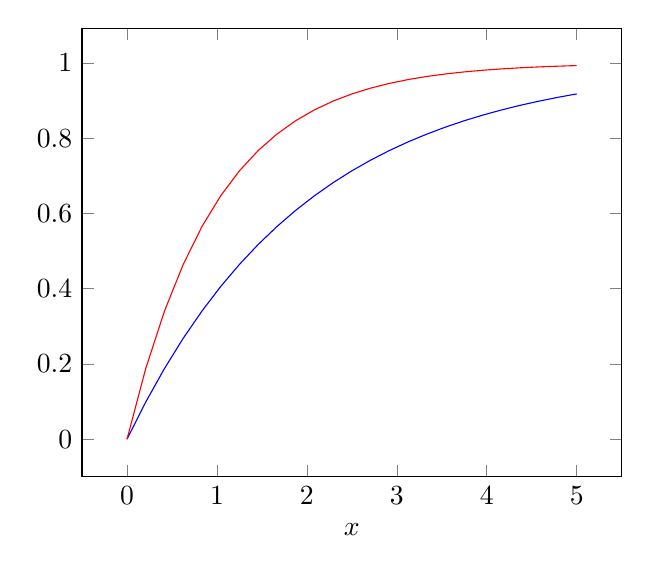
\begin{tikzpicture}[
            declare function={
                func(\x,\lambda) = (1 - e^(-\lambda*\x))
                ;
            }]
            \begin{axis}[xlabel=$x$]
                \addplot[blue][domain=0:5] {func(x,0.5)};
                \addplot[red][domain=0:5] {func(x,1)};
            \end{axis}
        \end{tikzpicture}
        \caption{$P(X \leq x)$ (funzione di ripartizione) di un'esponenziale di parametro $\lambda = 0.5$ (blu) e $\lambda = 1$ (rosso)}
        \label{exparam2}
    \end{figure}

    La funzione di ripartizione $ F $ è
    \begin{equation}
        F(x) = \int_{-\infty}^{x} f(t) dt = \begin{cases}
            0 & x \leq 0 \\
            1 - e^{-\lambda x} & x > 0 \\
        \end{cases}
    \end{equation}

\end{exmp}


\begin{note}
    Se X ha densità

    \begin{equation*}
        \p{X = x} = \int_x f(t) dt = 0
    \end{equation*}
\end{note}

\begin{defn}
    \textbf{Proprietà di una funzione di ripartizione} \\
    \begin{itemize}
        \item $s < t \implies F_X(1) \leq F_X(t)$ % TODO dim
        \item $\lim_{x \to -\infty} F(x) = 0$ \\
            $lim_{x \to +\infty} F(x) = 1$
        \item $F(x) = \lim_{y \to x^+} F(y)$
    \end{itemize}
\end{defn}

\section{Svolgere integrali multipli}
\begin{defn}
    \textbf{Integrale Multiplo} \\
    Un integrale multiplo è un integrale definito di una funzione a più di una
    variabile reale. Gli integrali di una funzione $f(x,y)$ su una regione di $ \R^2 $ sono detti
    \textbf{integrali doppi}, quelli di una funzione $f(x,y,z)$ su una regione di $ \R^3 $ sono detti \textbf{integrali tripli}.

    Proprio come l'integrale definito di una funzione positiva ad una variabile rappresenta
    l'area della regione sottostante al grafico della funzione, l'integrale doppio di
    una funzione positiva a due variabili reali rappresenta il volume della regione fra la superfice definita
    dalla funzione (sul piano cartesiano tridimensionale dove $ z = f(x, y)$) e il piano che contiene il dominio dell'integrale.
    Se sono presenti più variabili, un integrale multiplo produrrà ipervolumi di funzioni multidimensionali.
    L'integrazione multipla di una funzione ad $n$ variabili $f(x_1, x_2, \hdots, x_n)$ su un dominio $D$ è rappresentata
    da segni di integrale nidificati, nell'ordine inverso di esecuzione (l'integrale più a sinistra è calcolato per ultimo),
    seguita dalla funzione e i differenziali nell'ordine proprio (il segno di integrale più a sinistra corrisponde al differenziale
    più a destra). Il dominio di integrazione è rappresentato su ogni integrale, o simbolicamente abbreviato attraverso un simbolo
    di variabile sull'integrale più interno.
\end{defn}


\begin{defn}
    \textbf{Regola pratica per gli integrali doppi} \\
    \begin{equation}
        \iint_{\R^2} f(x,y) dx dy = \int_{\R} \left( \int_{\R} f(x,y) dy \right) dx = \int_{\R} dx \int_{\R} f(x,y) dy \\
        = \int_{\R} dy \int_{\R} f(x,y) dx
    \end{equation}
\end{defn}

\begin{exmp}
    \begin{figure}[htbp]
        \centering
        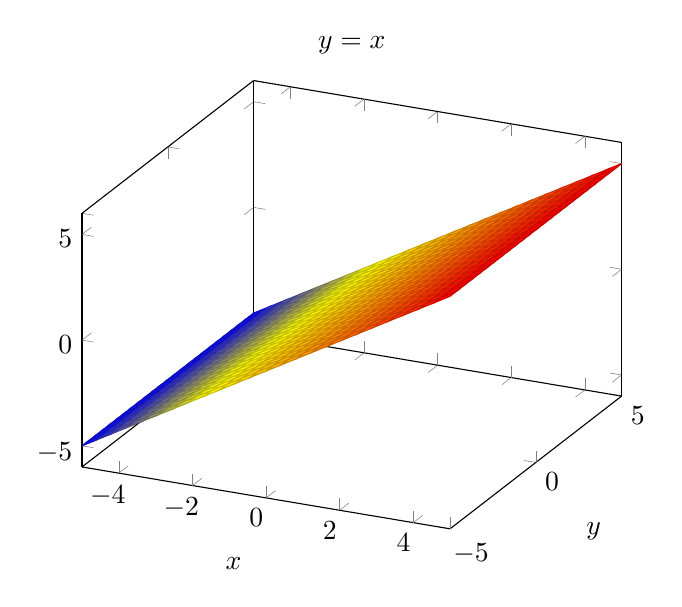
\begin{tikzpicture}
            \begin{axis}[
                title={$y = x$},
                xlabel=$x$, ylabel=$y$,
            ]
            \addplot3[
                surf,
                %domain=-2:2,
                %domain y=-1.3:1.3,
            ]
                {x};
            \end{axis}
            \end{tikzpicture}
        \caption{Grafico della funzione $y = x$ su $\R^2$}
        \label{2varplot}
    \end{figure}
    Svolgiamo l'integrale doppio sul triangolo $ T = 0 \leq y \leq x \leq 1$ di $f(x,y) = x$
    \begin{equation*}
        \begin{aligned}
            \iint_T x dydx = \int_0^1 \int_0^x x dydx = \int_0^1 dx \int_0^x x dy = \int_0^1 x^2 dx = \frac{1}{3} \\
        \end{aligned}
    \end{equation*}
    Che coincide, scambiando l'ordine di integrazione con
    \begin{equation*}
        \begin{aligned}
            \int_0^1 dy \int_y^1 x dx = \frac{1}{2} \int_0^1 (1-y^2) dy = \frac{1}{2} - \frac{1}{6} = \frac{1}{3}
        \end{aligned}
    \end{equation*}

\end{exmp}

\begin{exmp}
    \begin{figure}[htbp]
        \centering
        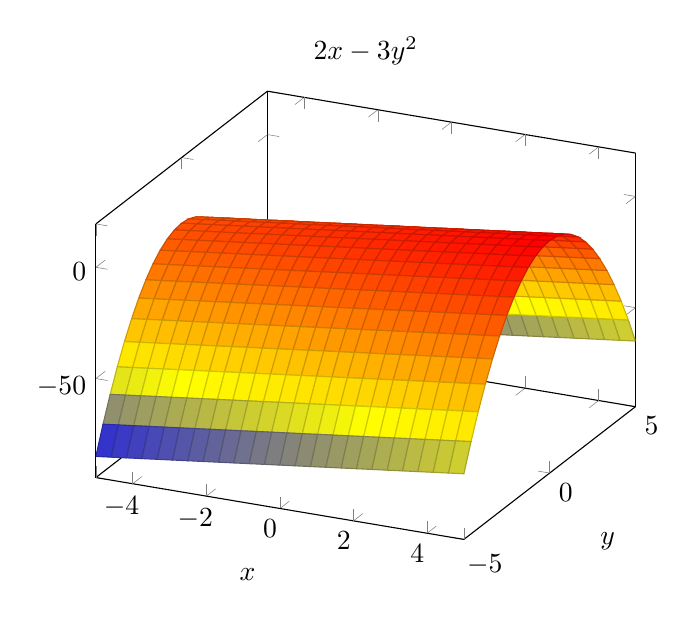
\begin{tikzpicture}
            \begin{axis}[
                title={$2x-3y^2$},
                xlabel=$x$, ylabel=$y$,
            ]
            \addplot3[
                surf,
                %domain=-2:2,
                %domain y=-1.3:1.3,
            ]
                {2*x-3*y^2};
            \end{axis}
            \end{tikzpicture}
        \caption{Grafico della funzione reale a due variabili $2x-3y^2$}
        \label{2varplot2}
    \end{figure}
    Svolgiamo l'integrale doppio $\iint_R 2x-3y^2 dx dy$ sul rettangolo $R: -1 \leq x \leq 1, 0 \leq y \leq 2$.

    \begin{equation*}
        \begin{aligned}
            \iint_R 2x-3y^2 dx dy = \int_0^2 \left( \int_{-1}^1 2x - 3y^2 dx \right) dy = \\
            \int_0^2 -6y^2 dy = (-6* \frac{8}{3}) = -16
        \end{aligned}
    \end{equation*}

\end{exmp}

\begin{defn}
    \textbf{Indipendenza di variabili continue}
    % TODO
\end{defn}

\begin{exrc}
    %TODO esercizio 3.1 (?)
\end{exrc}

% TODO recupera 12/11/19
% TODO recupera 14/11/19
% TODO recupera 19/11/19